\section{Experimental design}\label{sec:design}
Table~\ref{tab:studies} separates observation regimes and training variation. All studies use Meta-World~\cite{metaworld} 3.1.1/MuJoCo 3.3.0, a native 500-step horizon and mean native reward $U\in[0,10]$. Any-success records at least one native success event; terminal-success records the final step. Option branches and repeated policies are not independent environments. Online Resource 1 retains full training, condition, replay and provenance details.
\begin{table}[tb]\centering\small
\caption{Study roles and distinct observation/training regimes. Test counts are independent initial environments, not option branches or model--environment records. Actors and critic seeds vary different components. The full visual replication reuses 40 original development initial environments across three systems.}\label{tab:studies}
\setlength{\tabcolsep}{3pt}
\begin{tabular}{p{3.1cm}p{3.5cm}p{2.9cm}r}\toprule Study & Tasks / observations & Training variation & Test $n$\\\midrule
Original visual & Push, PickPlace / RGB+robot & Actor seed 0 & 500\\
Critic-data curve & Same visual tasks & Critic data 7/14/28 & 200\\
Full visual replication & Same visual tasks & Full systems 0/1/2 & 100\\
State stress suite & Drawer, Door, Button / state & Five critic seeds & 360\\
State channels & Same state tasks & Same frozen critics & 180\\
Visual channels & PickPlace / RGB+robot & Frozen original seed 0 & 60\\
Decoder control & PickPlace / RGB+robot & Same models; changed executor & 60\\\bottomrule
\end{tabular}
\end{table}


\subsection{Visual policies and development}
Push and PickPlace actors receive a vertically flipped $512\times512$ corner4 RGB image and four robot coordinates, without online object/goal poses. The ACT source~\cite{act} uses a pinned public pretrained initialization and produces 100 four-dimensional actions; it is not language-conditioned. Four local action/pose heads share a frozen ResNet-18 encoder. Each task supplies the same 200 demonstrations, split by whole episode into 180 training and 20 validation. Heads train for 20 epochs; ACT trains for 15,000 updates with validation-only checkpoint selection. Deployment capacities remain fixed. Pose heads receive additional offline supervision, so this is not an equal-information architecture comparison.

The original source reached any-success in 79/100 Push and 83/100 PickPlace qualification episodes, versus 91/100 and 90/100 for the selected local controllers. This establishes competence, not occasional-advice value. The seven local options comprise reject, three alternative feedback heads, an ensemble and request/arrival action holds; the full family adds five ACT prefix/suffix/blend options. Online Resource 1 specifies their execution rules.

The original arrival pool has 20 independent development episodes/task (14 training, six validation). Standard RBF kernel ridge critics predict option gains from request/arrival feature maps, robot coordinates, all head predictions and clocks; $P$ adds the full packet. Validation selects among 12 bandwidth/ridge combinations and zero. A $10^{-12}$ global-MSE tie tolerance favors zero; deployment requires predicted gain above $10^{-12}$. Actors and all four $L/P\times C/F$ critics are frozen before testing. Counterfactual rendering uses MSAA0 to remove observed same-state image variation; historical training features used MSAA4. This recorded change remains a distribution limitation.

\subsection{State policies and stress conditions}\label{sec:state-design}
Drawer, Door and Button cover sliding, hinged motion and pressing. They use ten public coordinates (hand, gripper, object and goal), a deterministic public scripted source and a nearest-neighbor behavioral-cloning local controller, rather than visual ACT. A preassigned demonstration ladder selects 40 episodes/task and $k=1,5,1$ using separate validation. Independent qualification requires both actors' any-success at least 0.8 on 20 environments; all three tasks pass and remain included.

Each task supplies 42 single-arrival development episodes (30/12 split). Six local options comprise reject, two alternative feedback policies and three action holds; four additional options hold or blend the source action. Five independently initialized 64/32 tanh critics per input/action cell train for 1,000 updates with validation checkpoint selection and an eligible zero predictor. Feature dimensions are 58/62; the tie tolerance is $10^{-12}$ and acceptance threshold $10^{-8}$. These are critic seeds around fixed actors, not independent actor-training systems.

A separate 360-environment stress suite crosses delays 0/16/64, single/periodic requests and position-noise standard deviations 0/0.005 m (120 environments/task). Noise affects nine position coordinates, with common time-indexed streams across branches. Periodic requests cannot overlap intervention windows. Packet zeroing, negation and reversal are gate-sensitivity probes only: no rerolled outcome or in-distribution interpretation is assigned to them.

\subsection{Fixed-policy channel studies}\label{sec:channelsetup}
Both channel studies freeze the trained receiver, normalization, thresholds, option functions and continuation. A common local prefix reaches the same arrival snapshot. Stale $c_s$ uses the source's request observation; fresh $c_f$ applies the same source to the arrival observation; absent $c_\emptyset$ invokes the fixed reject wrapper in Eq.~\eqref{eq:wrapper}. Messages are generated by the actual source, never arbitrary zero packets. Nonmessage inputs and request/delay clocks stay fixed. No extra refresh latency or acquisition cost is charged. Actual source generation does not ensure joint-input support under stale-only training.

The state study reuses all 60 critics on 60 fresh environments/task: delays 0/16/64 crossed with noise 0/0.005 m, ten per cell; a preassigned request occurs at 16/144/272/400. Every stale option and each distinct fresh source option is executed. The visual bridge instead fixes the \emph{original} seed-0 PickPlace system, connecting the null $P,C$ counterexample and the nonzero $P,F$ receiver. Its primary 60 fresh environments all have nonzero delay: 16/32 crossed with requests 16/32/64, ten per cell. Six separate delay-zero identity cases and two engineering cases are excluded from inference. Only distinct chosen plans and reject are executed, without a new oracle sweep.

For visual $c_f$, literal packet replacement retains the original option decoder, including suffix index $d+\text{elapsed}$. It does not reset fresh-message age or optimize a refresh controller. The contrast therefore tests this fixed receiver's content replacement, not the best possible refresh mechanism. Full 500-step rewards, actions and native success flags are retained. Channel choices are recorded before future outcomes; $R$ is independently replayed in every case. Decision changes and complete action differences above $10^{-8}$ are counted separately.

\subsection{Independent generation-time decoder control}\label{sec:decodersetup}
A separate experiment tests execution semantics on 60 new PickPlace environments, using the original seed-0 actors and critics without retraining. Delays 16/32 cross requests 16/32/64, with ten environments per cell; six zero-delay identities and two engineering cases are excluded. For a message generated at $g$, the time-matched suffix/blend decoder uses $(a-g)+\text{elapsed}$. Stale messages have $g=q$, reproducing the original index; refreshed messages have $g=a$, starting at zero. Raw-prefix and local options are unchanged. For the fixed 48-step option, time-matched fresh execution is the existing fresh raw-prefix candidate, not a new controller.

We evaluate both a predeclared fixed 48-step source suffix and the frozen $P,F$ gate. The gate receives unchanged packet/nonmessage features and selects the same option for both fresh decoders; only the downstream execution index changes. The four primary paired reward contrasts compare time-matched fresh execution against legacy fresh and legacy stale execution, separately for the fixed option and gate. Thirty thousand whole-environment bootstrap resamples within the six cells give approximate 98.75\% intervals for this independent four-contrast family. Secondary success and reject comparisons are descriptive.

This changes the executable receiver and therefore is an independent decoder-policy comparison, not a reinterpretation of the original fixed-policy channel effect. Since stale decoding is unchanged, fresh-versus-stale also measures refreshing under the newly defined timestamp-aware rule. The critic remains fitted to legacy outcomes; neither age-aware retraining nor optimal source timing is tested. Known, correct generation timestamps are assumed. No extra refresh latency or service cost is charged. Online Resource 1 retains the complete protocol, outcomes and index checks.

\subsection{Training variation and supporting studies}\label{sec:fullseedsetup}
The complete visual replication retains seed 0 and independently trains seeds 1/2, including ACT's full 15k budget, all four local heads and separately fitted 14/6 arrival critics. All share the immutable demonstration corpus, pretrained initialization, capacities and original development environment/clock arrangement. New actors generate their own development labels. This tests conditional training randomness, not cross-dataset or cross-task-distribution generalization.

Fifty fresh initial environments/task are shared by the three systems (100 independent initial environments, 300 system--environment cases). Every system also executes separate reset-source trajectories; none is excluded for weak competence. All 12 options are executed on the first ten preassigned environments/task per system for offline headroom. Figure~\ref{fig:scenes} illustrates excluded engineering cases rather than selected successful test episodes.

Supporting studies retain the original 250-environment/task visual confirmation, a new nested 7/14/28-episode critic-data curve with 100 fresh tests/task, and 100 development resplits across five tie tolerances. The earlier 3k source-budget studies are historical controls in Online Resource 1, not the full replication.

\subsection{Statistics, audit and research execution}\label{sec:statistics}
Comparisons retain whole-environment pairing. Stratified bootstrap resamples environments within preassigned cells; crossed versions additionally resample actor or critic seeds, never treating options as independent. The inference contract in Online Resource 1 gives every primary family, sample size and confidence level. These approximate percentile intervals have limited coverage with few training seeds or sparse differences; separate studies do not supply a global family guarantee. Native success, subgroup breakdowns and headroom are descriptive. The investigator-defined 0.25 reward reference has no validated operational meaning. Nonzero-delay state subsets are explicitly post-hoc, with exploratory 95\% intervals.

Frozen model/entry hashes, source consistency, raw reward means and recorded decisions are audited. Native restoration includes integration, task, observation-history and random state; local replay does not establish clean-machine portability. Source schedules, failed-run records and exact checks are retained in Online Resource 1. OpenAI Codex assisted implementation, orchestration, aggregation, literature checking and drafting beyond copy editing. Automated audits are not independent human verification; authors must verify and take responsibility for the final work.

\begin{figure}[tb]\centering
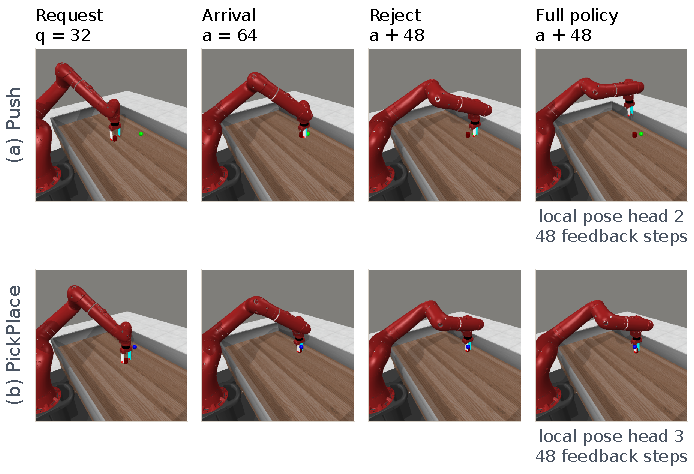
\includegraphics[width=\textwidth]{figures/simulator_scenes.pdf}
\caption{Preassigned engineering episodes, excluded from inference. Local control continues from request $q=32$ to arrival $a=64$. Final columns compare reject and $P,F$ at $a+48$. The policies select local pose heads 2 (Push) and 3 (PickPlace), not source actions. Each scene panel is rotated by $180^{\circ}$ for display; no crop or other pixel adjustment is applied. These are timing/branching examples, not efficacy evidence.}\label{fig:scenes}
\end{figure}
